\date{}
\title{}
\date{}
\begin{document}
\begin{frame}
    \titlepage
\end{frame}

\begin{frame}{revisiting congestion collapse}
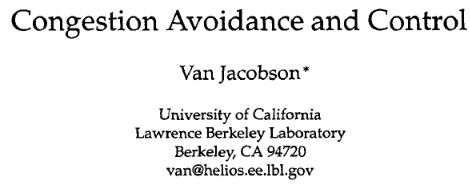
\includegraphics[width=0.6\textwidth]{../congest/jacobson-title}
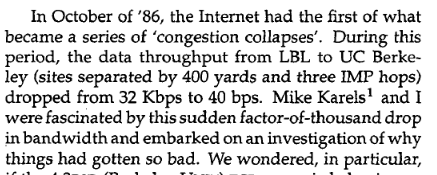
\includegraphics[width=0.6\textwidth]{../congest/jacobson-disaster}
\end{frame}

\begin{frame}<1>[label=jacobsonFixes]{fixes from Jacobson's 1987 paper}
\begin{tikzpicture}
\node[anchor=north west] (fixes) at (0, 0) {
    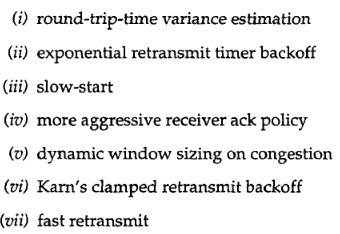
\includegraphics[width=0.6\textwidth]{../congest/jacobson-fixes}
};
%\path[draw,help lines] (0, 0) grid[step=1] (8, -5);
\begin{visibleenv}<2>
    \draw[red,ultra thick] (0, -3.8) rectangle (9, -4.4);
\end{visibleenv}
\begin{visibleenv}<4>
    \draw[red,ultra thick] (0, -2) rectangle (3, -2.8);
\end{visibleenv}
\begin{visibleenv}<3>
    \draw[red,ultra thick] (0, -5.4) rectangle (4.5, -6.2);
\end{visibleenv}
\end{tikzpicture}
\end{frame}


\begin{frame}
\frametitle{last time}
\begin{itemize}
\item ARP and duplicate IPs, intentional hijacking
\item DHCP --- get IP address + gateway by asking via broadcast
\item stateless autoconfiguration in IPv6
    \begin{itemize}
        \item choose arbitrary address within /64
    \end{itemize}
\item congestion collapse problem
    \begin{itemize}
    \item all flows lose when one flow overloads network
    \item retransmissions likely to make overload worse
    \end{itemize}
\end{itemize}
\end{frame}

\section{searching for performance}
\usetikzlibrary{arrows.meta,shapes.misc,shapes.geometric}
\begin{frame}{finding window size empirically (1)}
\begin{tikzpicture}
\draw[ultra thick,Latex-Latex] (-7, 0) -- (7, 0);
\draw[dotted,line width=2mm,violet] (1, 2) -- (1, -2) node[below] {capacity};
\node[align=left] at (-2, 0) {
    lowest latency \\
    (almost) no losses
};
\node[align=left] at (4.5, 0) {
    highest latency \\
    lots of losses 
};
\end{tikzpicture}
\end{frame}

\begin{frame}{key insight}
    \begin{itemize}
    \item latency/loss rate increases when window size too big
    \item latency/loss rate stable when window size not too big
    \vspace{.5cm}
    \item for now, we'll focus on loss rate
        \begin{itemize}
        \item but you can do something similar with latency
        \end{itemize}
    \end{tiemize}
\end{frame}

\begin{frame}{try a bunch of things}
\begin{tikzpicture}
\tikzset{
    good/.style={draw,star,thick,fill=green!70!black},
    bad/.style={draw,cross out,red!70!black,line width=3mm},
}
\draw[ultra thick,Latex-Latex] (-7, 0) -- (7, 0);
\node at (0, -.5) {window size};
\node[good,label={east:= low loss rate}] (key good) at (-6, 2) {};
\node[bad,label={east:= high loss rate}] (key bad) at (-6, 1) {};
\begin{visibleenv}<2->
\node[good] at (-3, 0){};
\node[bad] (high bad) at (5, 0){};
\end{visibleenv}
\begin{visibleenv}<3->
\node[bad] at (1, 0){}; 
\end{visibleenv}
\begin{visibleenv}<4->
\node[good] at (-1, 0){}; 
\end{visibleenv}
\begin{visibleenv}<5->
\node[good] at (-0.5, 0){}; 
\node[good] at (-0.2, 0){}; 
\node[bad] at (0.3, 0){}; 
\node[bad] at (0.5, 0){}; 
\node[bad] at (0.9, 0){}; 
\end{visibleenv}
\begin{visibleenv}<6>
\draw[Latex-,very thick] (high bad) -- ++(-2, -5) node {
    what is the network like when we do this?
};
\end{visibleenv}
\end{tikzpicture}
\end{frame}


\section{changing cross-traffic}

\usetikzlibrary{arrows.meta,calc,shapes}
\providecommand{\computer}{%
    
\includegraphics[width=1cm]{../common/Noun_project_216.pdf}
}
\providecommand{\switch}{%
    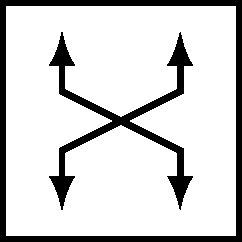
\includegraphics[width=0.9cm]{../common/fig-switch.pdf}
}
\providecommand{\router}{%
    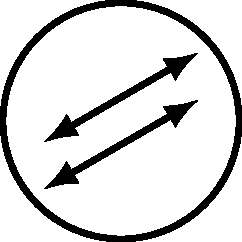
\includegraphics[width=0.9cm]{../common/fig-router.pdf}
}



\begin{frame}{changing cross-traffic}
\begin{tikzpicture}
\tikzset{
    computer/.style={inner sep=0mm,outer sep=0mm,execute at begin node={\computer}},
    switch/.style={inner sep=0mm,outer sep=0mm,execute at begin node={\switch}},
    router/.style={inner sep=0mm,outer sep=0mm,execute at begin node={\router},circle},
    connect/.style={draw,very thick,Latex-Latex},
    connect big/.style={draw,ultra thick,Latex-Latex},
}
\node[computer] (A) at (0, 0){};
\node[computer] (B) at (13, 0){};
\node[router] (r1) at (5, 0){};
\node[router] (r2) at (10, 0){};
\node[computer] (C) at (3, 3){};
\node[computer] (D) at (12, -3){};
\foreach \x/\y in {A/r1,r1/r2,r2/B,C/r1,r2/D} {
    \draw[connect] (\x) -- (\y);
}
\begin{visibleenv}<2>
\foreach \x/\y in {A/r1,r1/r2,r2/B} {
    \draw[blue,line width=1mm] ([yshift=-1mm]\x) -- ([yshift=-1mm]\y);
}
\node[text=blue,anchor=north] at ([yshift=-3mm]$(A)!0.5!(r1)$) {10Mbit};
\end{visibleenv}
\begin{visibleenv}<3>
\foreach \x/\y in {A.east/r1.west,r1.east/r2.west,r2.east/B.west} {
    \draw[-Latex,blue,line width=1mm] ([yshift=-3mm]\x) -- ([yshift=-3mm]\y);
}
\foreach \x/\y in {C/r1,r1.east/r2.west,r2/D} {
    \draw[-Latex,red,dotted,line width=1mm] ([yshift=3mm]\x) -- ([yshift=3mm]\y);
}
\node[text=blue,anchor=north] at ([yshift=-3mm]$(A)!0.5!(r1)$) {\sout{10Mbit} 7Mbit};
\node[text=red,anchor=west] at ($(C)!0.5!(r1)$) {3Mbit};
\end{visibleenv}
\begin{visibleenv}<4>
\foreach \x/\y in {A/r1,r1/r2,r2/B} {
    \draw[blue,line width=1mm] ([yshift=-1mm]\x) -- ([yshift=-1mm]\y);
}
\node[text=blue,anchor=north] at ([yshift=-3mm]$(A)!0.5!(r1)$) {\sout{10Mbit} \sout{7Mbit} 10Mbit};
\end{visibleenv}
\end{tikzpicture}
\end{frame}

\begin{frame}{adapting to cross-traffic}
    \begin{itemize}
    \item available bandwidth will change
    \item previous example: 3Mbit lost/added from other flow
    \vspace{.5cm}
    \item need to adapt to lost bandwidth
    \item need to detect new available bandwidth
    \end{itemize}
\end{frame}

\begin{frame}{other flow's bandwidth?}
    \begin{itemize}
    \item for now, we'll pretend other flows don't react to us
    \vspace{.5cm}
    \item later topic: what happens when both reacting?
    \end{itemize}
\end{frame}


\section{up/down pattern (rough)}
\begin{frame}{window size experimenting}
\begin{tikzpicture}
\tikzset{
    axis line/.style={draw,line width=1mm,-Latex},
    optimum/.style={draw,line width=0.5mm,dashed},
    actual/.style={draw,line width=0.75mm,violet,line to},
    down segment/.style={},
}
    \begin{scope}[y=.8cm,x=.9cm]
        \path[fill=red!10] (0, 6) rectangle (6, 8);
        \path[fill=red!10] (6, 4) rectangle (10, 8);
        \path[fill=red!10] (10, 6) rectangle (14, 8);
        \node[text=red!70!black] at (8, 7) {packets dropped sometimes};
        \node[text=green!70!black] at (8, 2) {packets not dropped};
        
        \path[actual]
            (0, 5.5) to
            (3, 6.3) coordinate (down1) to
            (3, 5.5) to
            (4, 5.8) to
            (6.1, 6.1) coordinate (down2) to
            (6.1, 5.7) to
            (6.5, 5.9) coordinate (down3) to
            (6.5, 5.5) to
            (6.7, 5.7) coordinate (down4) to
            (6.7, 4.8) to
            (6.8, 4.9) coordinate (down5) to
            (6.8, 3.7) to
            (7, 3.8) to
            (8, 4.2) coordinate (down6) to
            (8, 3.5) to
            (9, 3.7) to 
            (10, 4.1) to
            (11, 5.7) to
            (12.5, 6.2) coordinate (down7) to
            (12.5, 5.7) to
            (13, 5.8) to 
            (14, 6.1);

        \foreach \x in {1,...,7} {
            \node[draw=red,cross out,line width=2mm] at (down\x) {};
        };

        \path[axis line] (0, 0) -- (0, 8);
        \path[axis line] (0, 0) -- (14, 0);
        \node[anchor=north] at (7, 0) {time};
        \node[anchor=east,align=center] at (0, 4) {window\\size};
        \path[optimum] (0, 6) -- (6, 6);
        \path[optimum] (6, 4) -- (10, 4);
        \path[optimum] (10, 6) -- (14, 6);
        \begin{visibleenv}<2>
            \node[draw=red,fill=white,ultra thick,align=left,overlay,anchor=north] (up msg) at (3, 2) {
                always try increasing window size
            };
        \end{visibleenv}

        \begin{visibleenv}<3>
            \node[draw=red,fill=white,ultra thick,align=left,overlay,anchor=north] (drop msg) at (3, 2) {
                react to drops \\ by decreasing window
            };
            \foreach \x in {1,...,7} {
                \path[draw=red!50!black, very thick,-Latex] (drop msg) -- (down\x);
            }
        \end{visibleenv}
    \end{scope}
\end{tikzpicture}
\end{frame}

\begin{frame}{increase/decrease strategy}
    \begin{itemize}
    \item default to increasing window size
    \item react to packet drops by decreasing window size
        \begin{itemize}
        \item \myemph<2>{assumption: few ``non-congestion'' packet losses}
        \end{itemize}
    \vspace{.5cm}
    \item<3-> big topic: how fast to do each?
    \item<3-> questions to help decide that:
        \begin{itemize}
        \item what happens if we increase too fast? too slow?
        \item what happens if we decrease too fast? too slow?
        \end{itemize}
    \end{itemize}
\end{frame}

    % FIXME: show sawtooth pattern

\section{heuristic: slow increase}
\begin{frame}{slow increase}
    \begin{itemize}
    \item want to increase \textit{slowly} to avoid overload
    \item original TCP: +1 packet/round trip time
    \vspace{.5cm}
    \item<2-> +1 certainly not optimal choice, but okay heuristic
    \item<2-> important theoretically: approx. \myemph{additive} increase
        \begin{itemize}
        \item helps ensure good behavior with multiple connections
        \item (we'll talk later about why)
        \end{itemize}
    \end{itemize}
\end{frame}


\subsection{exercise: convergence times}
\begin{frame}{exercise: convergence time (1)}
    \begin{itemize}
    \item suppose: 50 ms round trip time
    \item initially sending at 600 packets/second
        \begin{itemize}
        \item $\approx 0.9$Mbyte/sec with 1500 byte packets
        \end{itemize}
    \item optimal rate is 10000 packets/second
        \begin{itemize}
        \item $\approx 15$Mbyte/sec with 1500 byte packets
        \end{itemize}
    \item `standard' TCP increase of 1 packet/RTT
    \item how long to get there?
    \item<2-> current: 30 packets/RTT (= window size 30)
    \item<2-> need to get to: 500 packets/RTT
    \item<2-> will take $500-30=470$ round trips $\approx$ 23500 ms $\approx$ 24 s
    \end{itemize}
\end{frame}

\begin{frame}{fixing bad convergence time}
    \begin{itemize}
    \item TCP's additive increase is very slow for ``high bandwidth-delay'' networks
    \item two things make this better:
    \vspace{.5cm}
    \item not in additive increase mode at start of connection
        \begin{itemize}
        \item ``slow start'' we'll talk about later
        \end{itemize}
    \item more adaptive increase for modern TCP variants
        \begin{itemize}
        \item e.g. FAST TCP, CUBIC TCP, \ldots
        \item heuristics to increase faster when appropriate
        \end{itemize}
    \end{itemize}
\end{frame}


\section{heuristic: fast decrease (v1)}
\begin{frame}{heurstic: fast decrease (v1)}
    \begin{itemize}
    \item want to decrease quickly to get out of overload
    \item original TCP heuristic: reset window to 1 packet
    \end{itemize}
\end{frame}


\section{original TCP congestion control}
\begin{frame}{TCP Tahoe}
    \begin{itemize}
    \item first version of TCP congestion control
    \item track two variables
        \begin{itemize}
        \item \texttt{cwnd} = congestion window
        \item \texttt{ssthresh} = `slow start threshold'
        \end{itemize}
    \item two modes of operation:
    \item \textit{congestion avoidance} (cwnd $\ge$ ssthresh; no known loss)
        \begin{itemize}
        \item represents ``steady state'' --- our focus for now
        \item no loss: cwnd += 1 segment per round-trip-time
        \item on loss: cwnd = $\sim$2 segments; ssthresh = cwnd/2
        \end{itemize}
    \item \textit{recovery} (known loss)
        \begin{itemize}
        \item retransmit packet after third duplicate ACK of previous packet :or timeout
        \end{itemize}
    \item \textit{``slow start''} (cwnd < ssthresh)
        \begin{itemize}
        \item intuition: not in ``steady state'' yet
        \item want to get there  quickly, but with overloading network
        \item we'll give details later
        \end{itemize}
    \end{itemize}
\end{frame}

\begin{frame}{plan}
    \begin{itemize}
    \item really don't want to reset to beginning on loss
        \begin{itemize}
        \item even if we have a way to get to good size quickly
        \end{itemize}
    \item would like to less extreme decrease: cwnd = cwnd/2
    \end{itemize}
\end{frame}


\section{part 1: window sizing}
\againframe<2>{jacobsonFixes}

\section{focus on steady state}
\begin{frame}{handling steady state}
    \begin{itemize}
    \item most of the time we should be at approx. correct window size
    \vspace{.5cm}
    \item want to focus on how we react to changes
    \item still going to use ``experimentation'' idea
    \end{itemize}
\end{frame}


\section{revised TCP congestion control}
\begin{frame}
\frametitle{TCP (New)Reno}
\begin{itemize}
    \item base for `modern' TCP (changes from Tahoe highlighted)
    \item \textit{congestion avoidance} (cwnd $\ge$ ssthresh; no known loss)
        \begin{itemize}
        \item no loss: cwnd += 1 segment per round-trip-time
        \item \myemph{on loss (dup ACK): cwnd = cwnd/2; ssthresh = new cwnd}
        \item on loss (timeout): cwnd = 2 segments
        \end{itemize}
    \item \textit{recovery} (known loss)
        \begin{itemize}
        \item resend immediately on third dup ACK
        \item \myemph{send new data based on self-clocking idea (``fast recovery'')}
        \end{itemize}
    \end{itemize}
\end{frame}


\section{heuristic: fast decrease (v2)}
\begin{frame}{fast decrease}
    \begin{itemize}
    \item want to decrease quickly to get out of overload
    \item original TCP heuristic: divide by two (minimum 1 packet)
    \vspace{.5cm}
    \item<2-> exactly by two probably not important
    \item<2-> important theoretically: approx. \myemph{multiplicative} decrease
        \begin{itemize}
        \item will help show okay behavior with multiple flows
        \end{itemize}
    \end{itemize}
\end{frame}

\begin{frame}{AIMD}
    \begin{itemize}
    \item additive increase + multiplicative decrease
    \item basic of steady-state behavior
    \end{itemize}
\end{frame}


\section{AIMD}

\begin{frame}{AIMD}
    \begin{itemize}
    \item result: additive increase + multiplicative decrease
    \vspace{.5cm}
    \item preview: good theoretical properties for \textit{sharing connections}
        \begin{itemize}
        \item doesn't matter much what additive/multiplicative factor is!
        \end{itemize}
    \item but: not quite what current Internet does
    \end{itemize}
\end{frame}


    % FIXME: hilite distance measurement oof down parts on sawtooth pattern

\section{some graphs}
\begin{frame}[label=vegasrenotrace]{}
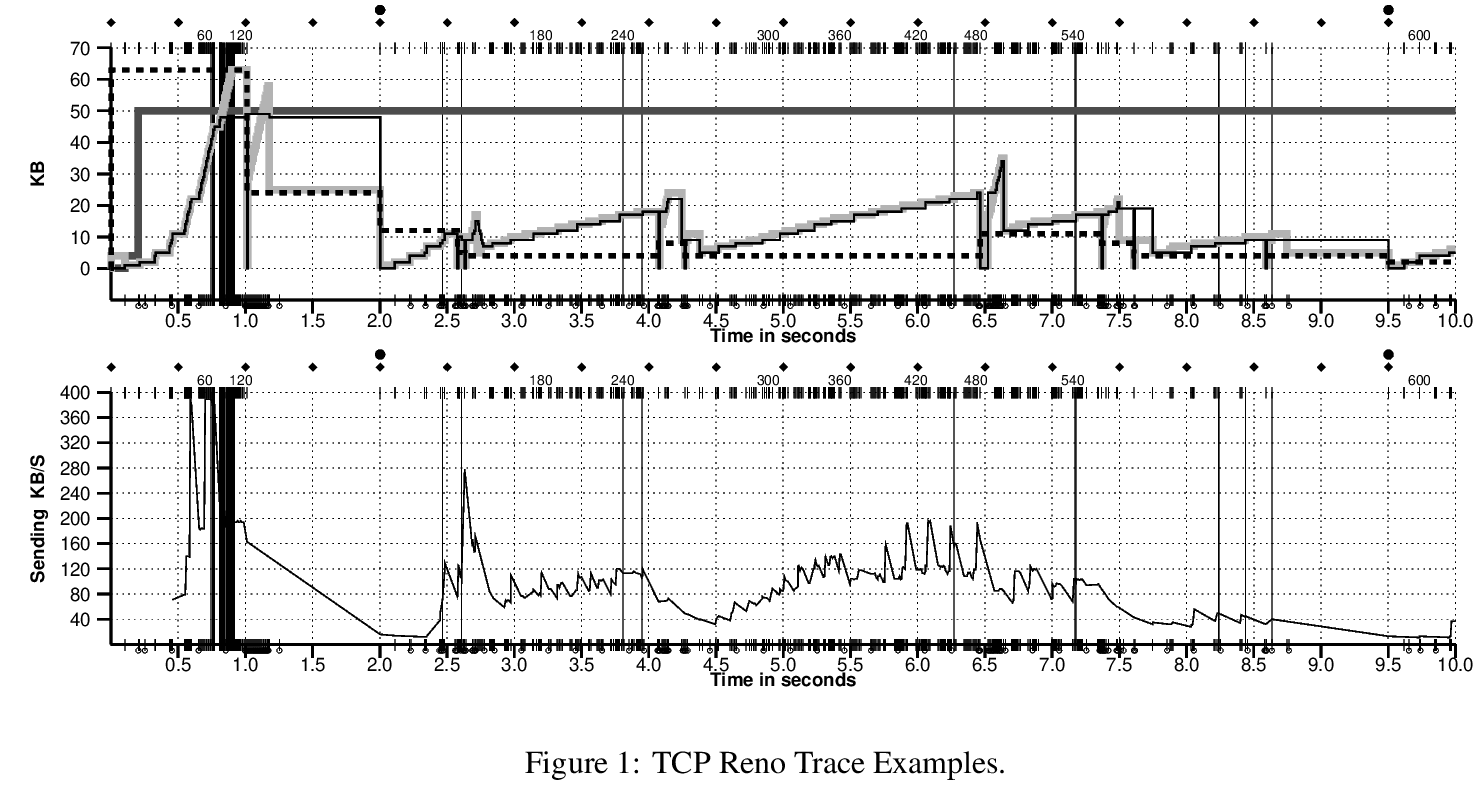
\includegraphics[width=0.9\textwidth]{../congest/vegas-fig1} \\
{
    \tiny from Brakmo, O'Malley, and Peterson, ``TCP Vegas: New techniques for
congestion detection and avoidance''} \\
    \small top thick, light-grey line = congestion window; dotted = slow start threshold
\end{frame}





\subsection{exercise: non-congestion losses} % FIXME: modify for decrease to 1
\begin{frame}{non-congestion losses}
    \begin{itemize}
    \item we were ignoring non-congestion losses
    \item suppose \myemph{1\%} loss rate from transmission errors
    \vspace{.5cm}
    \item 100 ms round trip time, very high bandwidth
    \item with TCP heuristics (+1 packet/RTT, half on loss)\ldots
    \item normal window size?
    \end{itemize}
\end{frame}



\section{backup slides}
\begin{frame}\frametitle{backup slides}
\end{frame}

\section{slow start later}

\begin{frame}{``slow start'' later}
    % FIXME: diagram
    \begin{itemize}
    \item heuristic: slow start if window size is `small' compared to last packet loss
        \begin{itemize}
        \item compromise: find correct size v. overload network
        \end{itemize}
    \vspace{.5cm}
    \item method:
    \item set \texttt{ssthresh} = bytes in flight / 2 on packet loss
    \item use slow start when window size < \texttt{ssthresh}
    \end{itemize}
\end{frame}



\end{document}
